% Suggested addition to the Reviewer 2 response.
% Figure path assumes the response is compiled from this package directory.
\noindent\textbf{Additional look-ahead-weight interaction analysis.}

In the R1-aligned implementation, the look-ahead congestion term weighted by $\omega$ is enabled only on Map A; Maps B and C use the Manhattan-distance heuristic without this term. We therefore evaluated the interactions involving $\omega$ on Map A only. The tested pairs were $\omega\times\sigma_l$, $\omega\times\sigma_t$, and $\omega\times K$, using $\omega\in\{10,50,100\}$, $\sigma_l,\sigma_t\in\{0.5,1,2,4\}$, and $K\in\{1,10,20,30,40\}$. The other parameters were held at the executable-source baseline, with $\sigma_t=2$ for $\omega\times\sigma_l$ and $\sigma_l=2$ for $\omega\times\sigma_t$.

The experiments used 50 and 70 tasks on Map A and five seeds (10000--10004). For every load--seed combination, the same task instance was reused across all parameter settings. The three grids contain 39 logical cells, with overlapping configurations reused, giving 33 unique configurations per load--seed combination and 330 complete one-shot CPS-A executions in total.

Figure~\ref{fig:r2-03-omega-interactions} reports high-load success-rate differences relative to the formal baseline. At $N=70$, the baseline success rate was 74.86\%. Across the tested grid, the changes ranged from $-4.57$ to $+3.43$ percentage points for $\omega\times\sigma_l$, from $-2.00$ to $+2.29$ points for $\omega\times\sigma_t$, and from $-4.29$ to $+4.00$ points for $\omega\times K$. Thus, the tested temporal-width interaction showed a narrower range of success-rate variation than the spatial-width and update-interval interactions. These results indicate that the influence of the look-ahead weight depends on its interaction with the spatial spread and update interval; they do not establish universal parameter insensitivity or statistical significance. The corresponding success-rate, planning-time, and average-path-length results for both loads are provided in the Supplementary Material.

\begin{figure}[!htbp]
    \centering
    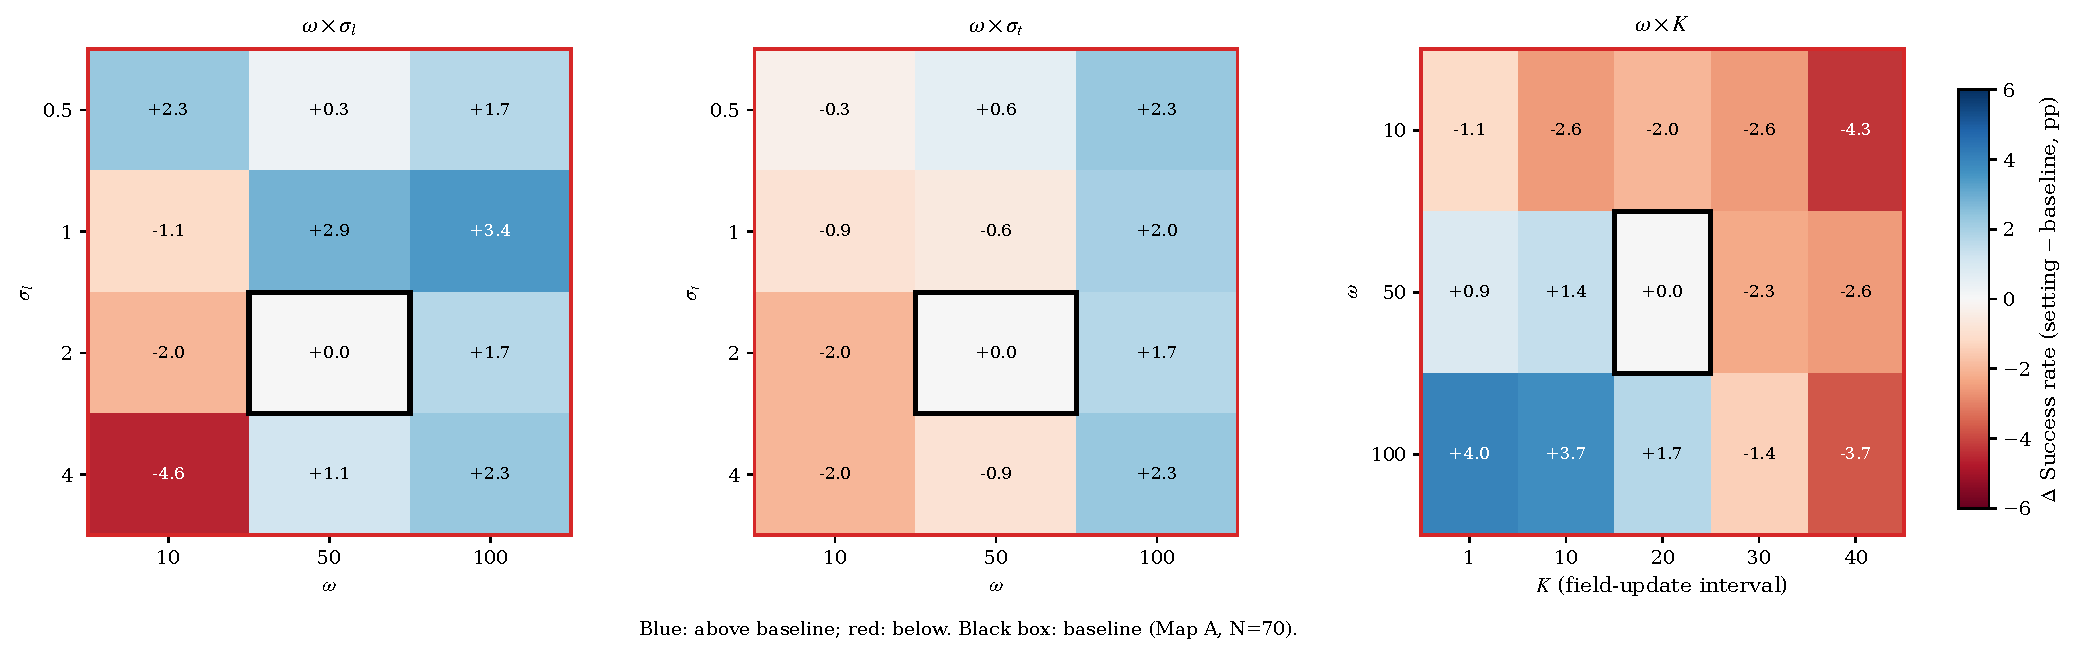
\includegraphics[width=\textwidth]{omega_interaction_figures/01_response_letter/Figure_R2_03_Response_Omega_Interactions.pdf}
    \caption{Look-ahead-weight interaction sensitivity on Map A.}
    \label{fig:r2-03-omega-interactions}
\end{figure}
